\documentclass[1p]{elsarticle_modified}
%\bibliographystyle{elsarticle-num}

%\usepackage[colorlinks]{hyperref}
%\usepackage{abbrmath_seonhwa} %\Abb, \Ascr, \Acal ,\Abf, \Afrak
\usepackage{amsfonts}
\usepackage{amssymb}
\usepackage{amsmath}
\usepackage{amsthm}
\usepackage{scalefnt}
\usepackage{amsbsy}
\usepackage{kotex}
\usepackage{caption}
\usepackage{subfig}
\usepackage{color}
\usepackage{graphicx}
\usepackage{xcolor} %% white, black, red, green, blue, cyan, magenta, yellow
\usepackage{float}
\usepackage{setspace}
\usepackage{hyperref}

\usepackage{tikz}
\usetikzlibrary{arrows}

\usepackage{multirow}
\usepackage{array} % fixed length table
\usepackage{hhline}

%%%%%%%%%%%%%%%%%%%%%
\makeatletter
\renewcommand*\env@matrix[1][\arraystretch]{%
	\edef\arraystretch{#1}%
	\hskip -\arraycolsep
	\let\@ifnextchar\new@ifnextchar
	\array{*\c@MaxMatrixCols c}}
\makeatother %https://tex.stackexchange.com/questions/14071/how-can-i-increase-the-line-spacing-in-a-matrix
%%%%%%%%%%%%%%%

\usepackage[normalem]{ulem}

\newcommand{\msout}[1]{\ifmmode\text{\sout{\ensuremath{#1}}}\else\sout{#1}\fi}
%SOURCE: \msout is \stkout macro in https://tex.stackexchange.com/questions/20609/strikeout-in-math-mode

\newcommand{\cancel}[1]{
	\ifmmode
	{\color{red}\msout{#1}}
	\else
	{\color{red}\sout{#1}}
	\fi
}

\newcommand{\add}[1]{
	{\color{blue}\uwave{#1}}
}

\newcommand{\replace}[2]{
	\ifmmode
	{\color{red}\msout{#1}}{\color{blue}\uwave{#2}}
	\else
	{\color{red}\sout{#1}}{\color{blue}\uwave{#2}}
	\fi
}

\newcommand{\Sol}{\mathcal{S}} %segment
\newcommand{\D}{D} %diagram
\newcommand{\A}{\mathcal{A}} %arc


%%%%%%%%%%%%%%%%%%%%%%%%%%%%%5 test

\def\sl{\operatorname{\textup{SL}}(2,\Cbb)}
\def\psl{\operatorname{\textup{PSL}}(2,\Cbb)}
\def\quan{\mkern 1mu \triangleright \mkern 1mu}

\theoremstyle{definition}
\newtheorem{thm}{Theorem}[section]
\newtheorem{prop}[thm]{Proposition}
\newtheorem{lem}[thm]{Lemma}
\newtheorem{ques}[thm]{Question}
\newtheorem{cor}[thm]{Corollary}
\newtheorem{defn}[thm]{Definition}
\newtheorem{exam}[thm]{Example}
\newtheorem{rmk}[thm]{Remark}
\newtheorem{alg}[thm]{Algorithm}

\newcommand{\I}{\sqrt{-1}}
\begin{document}

%\begin{frontmatter}
%
%\title{Boundary parabolic representations of knots up to 8 crossings}
%
%%% Group authors per affiliation:
%\author{Yunhi Cho} 
%\address{Department of Mathematics, University of Seoul, Seoul, Korea}
%\ead{yhcho@uos.ac.kr}
%
%
%\author{Seonhwa Kim} %\fnref{s_kim}}
%\address{Center for Geometry and Physics, Institute for Basic Science, Pohang, 37673, Korea}
%\ead{ryeona17@ibs.re.kr}
%
%\author{Hyuk Kim}
%\address{Department of Mathematical Sciences, Seoul National University, Seoul 08826, Korea}
%\ead{hyukkim@snu.ac.kr}
%
%\author{Seokbeom Yoon}
%\address{Department of Mathematical Sciences, Seoul National University, Seoul, 08826,  Korea}
%\ead{sbyoon15@snu.ac.kr}
%
%\begin{abstract}
%We find all boundary parabolic representation of knots up to 8 crossings.
%
%\end{abstract}
%\begin{keyword}
%    \MSC[2010] 57M25 
%\end{keyword}
%
%\end{frontmatter}

%\linenumbers
%\tableofcontents
%
\newcommand\colored[1]{\textcolor{white}{\rule[-0.35ex]{0.8em}{1.4ex}}\kern-0.8em\color{red} #1}%
%\newcommand\colored[1]{\textcolor{white}{ #1}\kern-2.17ex	\textcolor{white}{ #1}\kern-1.81ex	\textcolor{white}{ #1}\kern-2.15ex\color{red}#1	}

{\Large $\underline{10_{42}~(K10a_{31})}$}

\setlength{\tabcolsep}{10pt}
\renewcommand{\arraystretch}{1.6}
\vspace{1cm}\begin{tabular}{m{100pt}>{\centering\arraybackslash}m{274pt}}
\multirow{5}{120pt}{
	\centering
	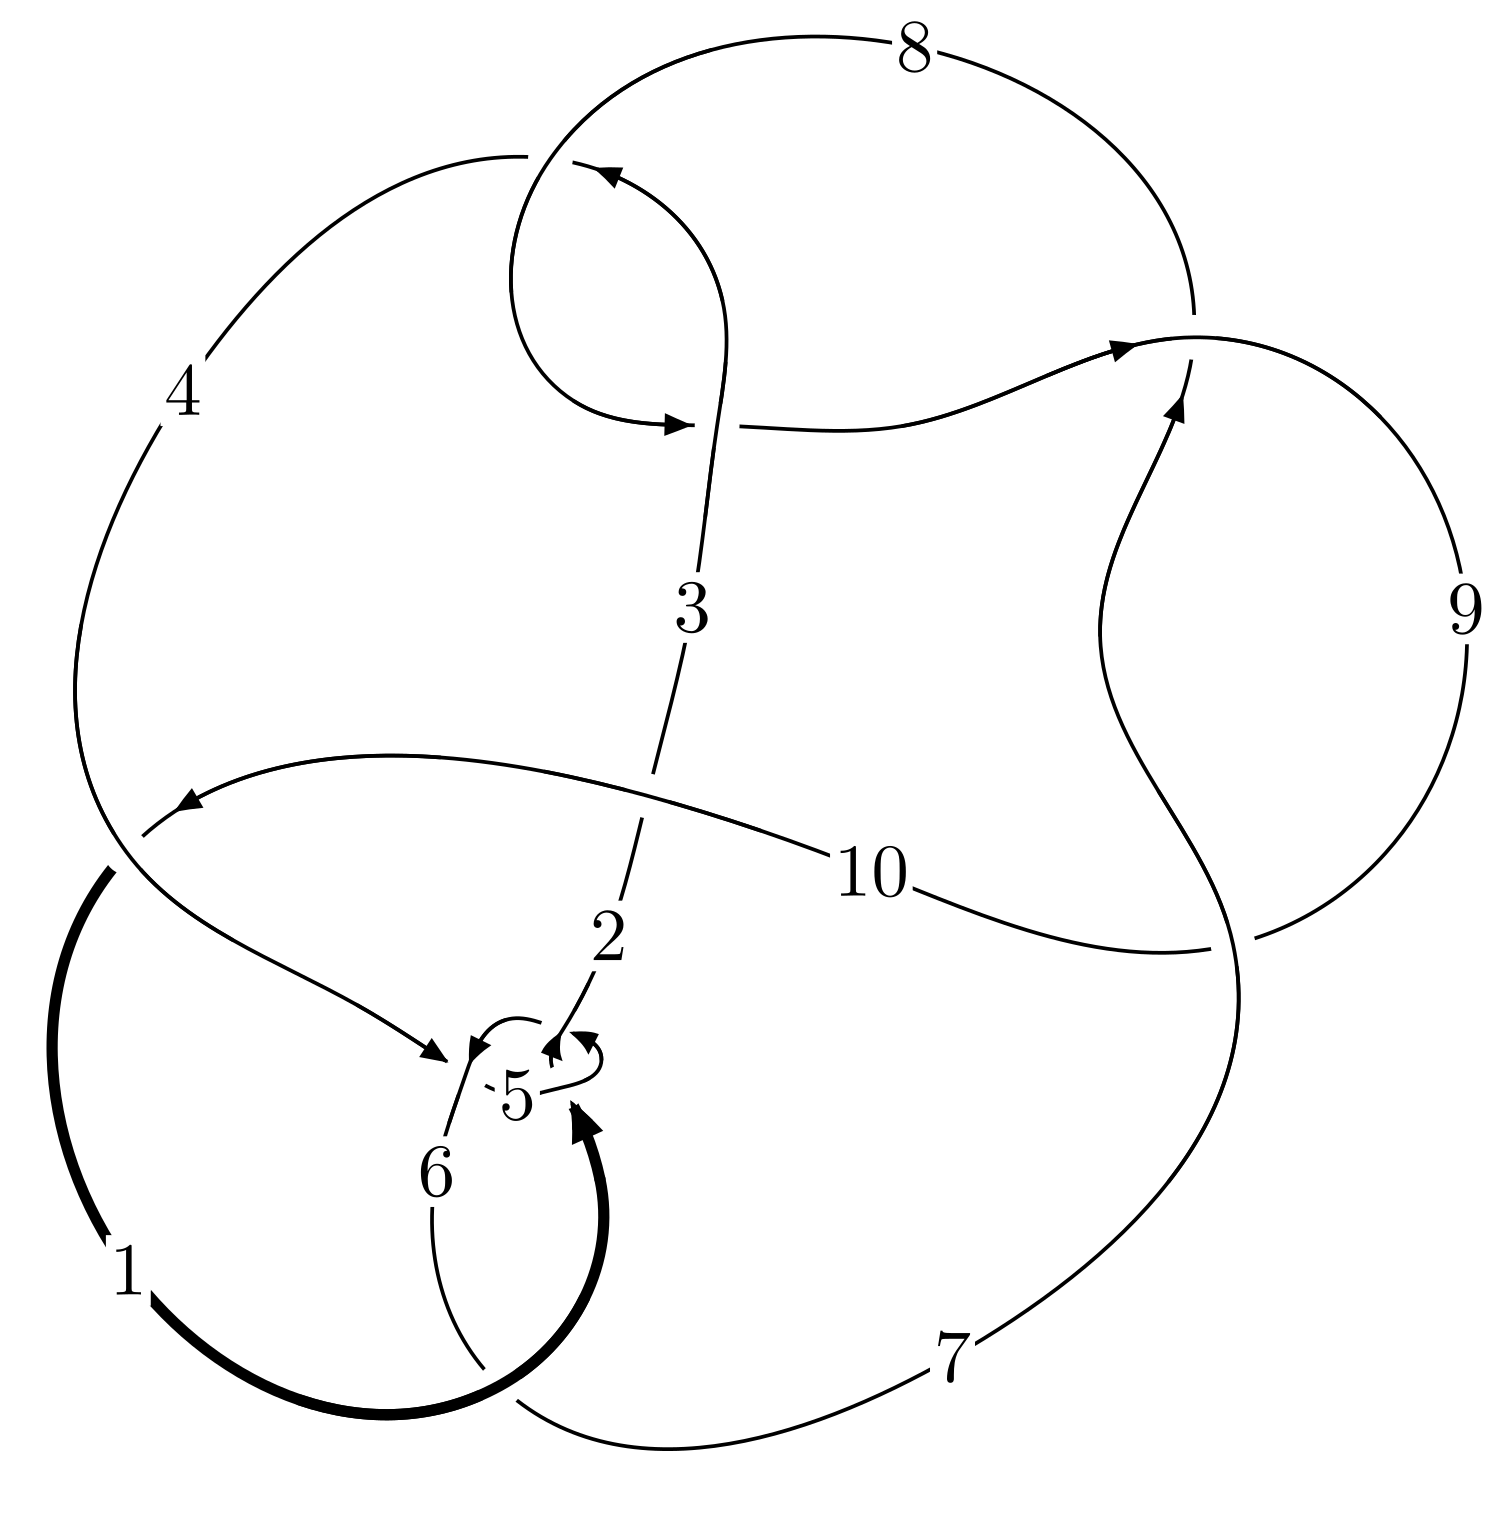
\includegraphics[width=112pt]{../../../GIT/diagram.site/Diagrams/png/126_10_42.png}\\
\ \ \ A knot diagram\footnotemark}&
\allowdisplaybreaks
\textbf{Linearized knot diagam} \\
\cline{2-2}
 &
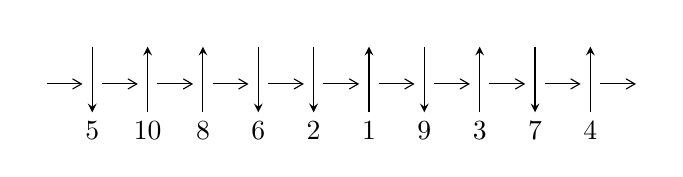
\begin{tikzpicture}[x=20pt, y=17pt]
	% nodes
	\node (C0) at (0, 0) {};
	\node (C1) at (1, 0) {};
	\node (C1U) at (1, +1) {};
	\node (C1D) at (1, -1) {5};

	\node (C2) at (2, 0) {};
	\node (C2U) at (2, +1) {};
	\node (C2D) at (2, -1) {10};

	\node (C3) at (3, 0) {};
	\node (C3U) at (3, +1) {};
	\node (C3D) at (3, -1) {8};

	\node (C4) at (4, 0) {};
	\node (C4U) at (4, +1) {};
	\node (C4D) at (4, -1) {6};

	\node (C5) at (5, 0) {};
	\node (C5U) at (5, +1) {};
	\node (C5D) at (5, -1) {2};

	\node (C6) at (6, 0) {};
	\node (C6U) at (6, +1) {};
	\node (C6D) at (6, -1) {1};

	\node (C7) at (7, 0) {};
	\node (C7U) at (7, +1) {};
	\node (C7D) at (7, -1) {9};

	\node (C8) at (8, 0) {};
	\node (C8U) at (8, +1) {};
	\node (C8D) at (8, -1) {3};

	\node (C9) at (9, 0) {};
	\node (C9U) at (9, +1) {};
	\node (C9D) at (9, -1) {7};

	\node (C10) at (10, 0) {};
	\node (C10U) at (10, +1) {};
	\node (C10D) at (10, -1) {4};
	\node (C11) at (11, 0) {};

	% arrows
	\draw[->,>={angle 60}]
	(C0) edge (C1) (C1) edge (C2) (C2) edge (C3) (C3) edge (C4) (C4) edge (C5) (C5) edge (C6) (C6) edge (C7) (C7) edge (C8) (C8) edge (C9) (C9) edge (C10) (C10) edge (C11) ;	\draw[->,>=stealth]
	(C1U) edge (C1D) (C2D) edge (C2U) (C3D) edge (C3U) (C4U) edge (C4D) (C5U) edge (C5D) (C6D) edge (C6U) (C7U) edge (C7D) (C8D) edge (C8U) (C9U) edge (C9D) (C10D) edge (C10U) ;
	\end{tikzpicture} \\
\hhline{~~} \\& 
\textbf{Solving Sequence} \\ \cline{2-2} 
 &
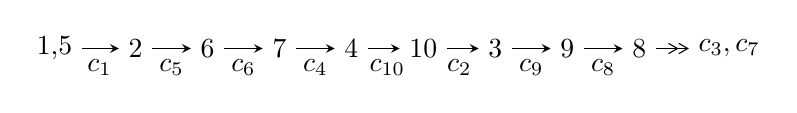
\begin{tikzpicture}[x=26pt, y=7pt]
	% node
	\node (A0) at (-1/8, 0) {1,5};
	\node (A1) at (1, 0) {2};
	\node (A2) at (2, 0) {6};
	\node (A3) at (3, 0) {7};
	\node (A4) at (4, 0) {4};
	\node (A5) at (5, 0) {10};
	\node (A6) at (6, 0) {3};
	\node (A7) at (7, 0) {9};
	\node (A8) at (8, 0) {8};
	\node (C1) at (1/2, -1) {$c_{1}$};
	\node (C2) at (3/2, -1) {$c_{5}$};
	\node (C3) at (5/2, -1) {$c_{6}$};
	\node (C4) at (7/2, -1) {$c_{4}$};
	\node (C5) at (9/2, -1) {$c_{10}$};
	\node (C6) at (11/2, -1) {$c_{2}$};
	\node (C7) at (13/2, -1) {$c_{9}$};
	\node (C8) at (15/2, -1) {$c_{8}$};
	\node (A9) at (37/4, 0) {$c_{3},c_{7}$};

	% edge
	\draw[->,>=stealth]	
	(A0) edge (A1) (A1) edge (A2) (A2) edge (A3) (A3) edge (A4) (A4) edge (A5) (A5) edge (A6) (A6) edge (A7) (A7) edge (A8) ;
	\draw[->>,>={angle 60}]	
	(A8) edge (A9);
\end{tikzpicture} \\ 

\end{tabular} \\

\footnotetext{
The image of knot diagram is generated by the software ``\textbf{Draw programme}" developed by Andrew Bartholomew(\url{http://www.layer8.co.uk/maths/draw/index.htm\#Running-draw}), where we modified some parts for our purpose(\url{https://github.com/CATsTAILs/LinksPainter}).
}\phantom \\ \newline 
\centering \textbf{Ideals for irreducible components\footnotemark of $X_{\text{par}}$} 
 
\begin{align*}
I^u_{1}&=\langle 
u^{40}+u^{39}+\cdots+2 u+1\rangle \\
\\
\end{align*}
\raggedright * 1 irreducible components of $\dim_{\mathbb{C}}=0$, with total 40 representations.\\
\footnotetext{All coefficients of polynomials are rational numbers. But the coefficients are sometimes approximated in decimal forms when there is not enough margin.}
\newpage
\renewcommand{\arraystretch}{1}
\centering \section*{I. $I^u_{1}= \langle u^{40}+u^{39}+\cdots+2 u+1 \rangle$}
\flushleft \textbf{(i) Arc colorings}\\
\begin{tabular}{m{7pt} m{180pt} m{7pt} m{180pt} }
\flushright $a_{1}=$&$\begin{pmatrix}1\\0\end{pmatrix}$ \\
\flushright $a_{5}=$&$\begin{pmatrix}0\\u\end{pmatrix}$ \\
\flushright $a_{2}=$&$\begin{pmatrix}1\\u^2\end{pmatrix}$ \\
\flushright $a_{6}=$&$\begin{pmatrix}- u\\- u^3+u\end{pmatrix}$ \\
\flushright $a_{7}=$&$\begin{pmatrix}- u^3\\- u^3+u\end{pmatrix}$ \\
\flushright $a_{4}=$&$\begin{pmatrix}u^3\\u^5- u^3+u\end{pmatrix}$ \\
\flushright $a_{10}=$&$\begin{pmatrix}u^8- u^6+u^4+1\\u^{10}-2 u^8+3 u^6-2 u^4+u^2\end{pmatrix}$ \\
\flushright $a_{3}=$&$\begin{pmatrix}u^{16}-3 u^{14}+5 u^{12}-4 u^{10}+3 u^8-2 u^6+2 u^4+1\\u^{18}-4 u^{16}+9 u^{14}-12 u^{12}+11 u^{10}-6 u^8+2 u^6+u^2\end{pmatrix}$ \\
\flushright $a_{9}=$&$\begin{pmatrix}u^{16}-3 u^{14}+5 u^{12}-4 u^{10}+3 u^8-2 u^6+2 u^4+1\\u^{16}-4 u^{14}+8 u^{12}-8 u^{10}+4 u^8\end{pmatrix}$ \\
\flushright $a_{8}=$&$\begin{pmatrix}- u^{29}+6 u^{27}+\cdots-4 u^5- u\\- u^{29}+7 u^{27}+\cdots- u^3+u\end{pmatrix}$\\&\end{tabular}
\flushleft \textbf{(ii) Obstruction class $= -1$}\\~\\
\flushleft \textbf{(iii) Cusp Shapes $= -4 u^{39}+40 u^{37}+4 u^{36}-200 u^{35}-36 u^{34}+644 u^{33}+164 u^{32}-1472 u^{31}-484 u^{30}+2500 u^{29}+1020 u^{28}-3236 u^{27}-1616 u^{26}+3252 u^{25}+2004 u^{24}-2608 u^{23}-2040 u^{22}+1752 u^{21}+1812 u^{20}-1036 u^{19}-1468 u^{18}+512 u^{17}+1064 u^{16}-160 u^{15}-652 u^{14}-16 u^{13}+340 u^{12}+72 u^{11}-168 u^{10}-96 u^9+68 u^8+76 u^7-8 u^6-24 u^5-4 u^4-4 u^3-4 u^2-8 u-6$}\\~\\
\newpage\renewcommand{\arraystretch}{1}
\flushleft \textbf{(iv) u-Polynomials at the component}\newline \\
\begin{tabular}{m{50pt}|m{274pt}}
Crossings & \hspace{64pt}u-Polynomials at each crossing \\
\hline $$\begin{aligned}c_{1},c_{5}\end{aligned}$$&$\begin{aligned}
&u^{40}+u^{39}+\cdots+2 u+1
\end{aligned}$\\
\hline $$\begin{aligned}c_{2}\end{aligned}$$&$\begin{aligned}
&u^{40}+5 u^{39}+\cdots+12 u+1
\end{aligned}$\\
\hline $$\begin{aligned}c_{3},c_{8}\end{aligned}$$&$\begin{aligned}
&u^{40}- u^{39}+\cdots-2 u^3+1
\end{aligned}$\\
\hline $$\begin{aligned}c_{4}\end{aligned}$$&$\begin{aligned}
&u^{40}+19 u^{39}+\cdots+2 u^2+1
\end{aligned}$\\
\hline $$\begin{aligned}c_{6}\end{aligned}$$&$\begin{aligned}
&u^{40}+3 u^{39}+\cdots+61 u+16
\end{aligned}$\\
\hline $$\begin{aligned}c_{7},c_{9}\end{aligned}$$&$\begin{aligned}
&u^{40}+13 u^{39}+\cdots-2 u^2+1
\end{aligned}$\\
\hline $$\begin{aligned}c_{10}\end{aligned}$$&$\begin{aligned}
&u^{40}- u^{39}+\cdots+70 u+25
\end{aligned}$\\
\hline
\end{tabular}\\~\\
\newpage\renewcommand{\arraystretch}{1}
\flushleft \textbf{(v) Riley Polynomials at the component}\newline \\
\begin{tabular}{m{50pt}|m{274pt}}
Crossings & \hspace{64pt}Riley Polynomials at each crossing \\
\hline $$\begin{aligned}c_{1},c_{5}\end{aligned}$$&$\begin{aligned}
&y^{40}-19 y^{39}+\cdots+2 y^2+1
\end{aligned}$\\
\hline $$\begin{aligned}c_{2}\end{aligned}$$&$\begin{aligned}
&y^{40}+y^{39}+\cdots+12 y+1
\end{aligned}$\\
\hline $$\begin{aligned}c_{3},c_{8}\end{aligned}$$&$\begin{aligned}
&y^{40}+13 y^{39}+\cdots-2 y^2+1
\end{aligned}$\\
\hline $$\begin{aligned}c_{4}\end{aligned}$$&$\begin{aligned}
&y^{40}+5 y^{39}+\cdots+4 y+1
\end{aligned}$\\
\hline $$\begin{aligned}c_{6}\end{aligned}$$&$\begin{aligned}
&y^{40}+9 y^{39}+\cdots+4695 y+256
\end{aligned}$\\
\hline $$\begin{aligned}c_{7},c_{9}\end{aligned}$$&$\begin{aligned}
&y^{40}+29 y^{39}+\cdots-4 y+1
\end{aligned}$\\
\hline $$\begin{aligned}c_{10}\end{aligned}$$&$\begin{aligned}
&y^{40}-11 y^{39}+\cdots-11300 y+625
\end{aligned}$\\
\hline
\end{tabular}\\~\\
\newpage\flushleft \textbf{(vi) Complex Volumes and Cusp Shapes}
$$\begin{array}{c|c|c}  
\text{Solutions to }I^u_{1}& \I (\text{vol} + \sqrt{-1}CS) & \text{Cusp shape}\\
 \hline 
\begin{aligned}
u &= -1.028980 + 0.356861 I\end{aligned}
 & -1.87833 + 1.42866 I & -1.75477 - 0.64534 I \\ \hline\begin{aligned}
u &= -1.028980 - 0.356861 I\end{aligned}
 & -1.87833 - 1.42866 I & -1.75477 + 0.64534 I \\ \hline\begin{aligned}
u &= -0.605776 + 0.668794 I\end{aligned}
 & \phantom{-}4.58827 + 5.88166 I & \phantom{-}4.65065 - 6.09482 I \\ \hline\begin{aligned}
u &= -0.605776 - 0.668794 I\end{aligned}
 & \phantom{-}4.58827 - 5.88166 I & \phantom{-}4.65065 + 6.09482 I \\ \hline\begin{aligned}
u &= -1.085730 + 0.202553 I\end{aligned}
 & -0.384043 - 0.065531 I & -1.65195 - 0.65182 I \\ \hline\begin{aligned}
u &= -1.085730 - 0.202553 I\end{aligned}
 & -0.384043 + 0.065531 I & -1.65195 + 0.65182 I \\ \hline\begin{aligned}
u &= \phantom{-}0.571687 + 0.673264 I\end{aligned}
 & \phantom{-}5.18330 - 0.15085 I & \phantom{-}6.02823 + 0.49618 I \\ \hline\begin{aligned}
u &= \phantom{-}0.571687 - 0.673264 I\end{aligned}
 & \phantom{-}5.18330 + 0.15085 I & \phantom{-}6.02823 - 0.49618 I \\ \hline\begin{aligned}
u &= -0.964797 + 0.581212 I\end{aligned}
 & \phantom{-}3.52924 - 1.02826 I & \phantom{-}3.02738 + 0.15735 I \\ \hline\begin{aligned}
u &= -0.964797 - 0.581212 I\end{aligned}
 & \phantom{-}3.52924 + 1.02826 I & \phantom{-}3.02738 - 0.15735 I \\ \hline\begin{aligned}
u &= \phantom{-}1.120660 + 0.212549 I\end{aligned}
 & -1.32786 + 5.57768 I & -3.43862 - 4.39035 I \\ \hline\begin{aligned}
u &= \phantom{-}1.120660 - 0.212549 I\end{aligned}
 & -1.32786 - 5.57768 I & -3.43862 + 4.39035 I \\ \hline\begin{aligned}
u &= \phantom{-}1.110950 + 0.292389 I\end{aligned}
 & -6.07985 - 0.03674 I & -9.04849 - 0.16943 I \\ \hline\begin{aligned}
u &= \phantom{-}1.110950 - 0.292389 I\end{aligned}
 & -6.07985 + 0.03674 I & -9.04849 + 0.16943 I \\ \hline\begin{aligned}
u &= \phantom{-}0.991959 + 0.580881 I\end{aligned}
 & \phantom{-}3.94345 - 4.71182 I & \phantom{-}3.76114 + 5.41408 I \\ \hline\begin{aligned}
u &= \phantom{-}0.991959 - 0.580881 I\end{aligned}
 & \phantom{-}3.94345 + 4.71182 I & \phantom{-}3.76114 - 5.41408 I \\ \hline\begin{aligned}
u &= -0.355458 + 0.766083 I\end{aligned}
 & \phantom{-}3.32299 - 8.17729 I & \phantom{-}3.05192 + 5.82128 I \\ \hline\begin{aligned}
u &= -0.355458 - 0.766083 I\end{aligned}
 & \phantom{-}3.32299 + 8.17729 I & \phantom{-}3.05192 - 5.82128 I \\ \hline\begin{aligned}
u &= \phantom{-}0.374958 + 0.750172 I\end{aligned}
 & \phantom{-}4.20581 + 2.43691 I & \phantom{-}4.87403 - 0.79132 I \\ \hline\begin{aligned}
u &= \phantom{-}0.374958 - 0.750172 I\end{aligned}
 & \phantom{-}4.20581 - 2.43691 I & \phantom{-}4.87403 + 0.79132 I \\ \hline\begin{aligned}
u &= \phantom{-}1.112780 + 0.379878 I\end{aligned}
 & -3.07700 - 5.78108 I & -4.88901 + 6.61715 I \\ \hline\begin{aligned}
u &= \phantom{-}1.112780 - 0.379878 I\end{aligned}
 & -3.07700 + 5.78108 I & -4.88901 - 6.61715 I \\ \hline\begin{aligned}
u &= -1.093860 + 0.474186 I\end{aligned}
 & -2.46460 + 1.67611 I & -4.01967 - 0.72581 I \\ \hline\begin{aligned}
u &= -1.093860 - 0.474186 I\end{aligned}
 & -2.46460 - 1.67611 I & -4.01967 + 0.72581 I \\ \hline\begin{aligned}
u &= \phantom{-}1.075660 + 0.536322 I\end{aligned}
 & -0.51656 - 5.28641 I & \phantom{-}1.70674 + 5.92677 I \\ \hline\begin{aligned}
u &= \phantom{-}1.075660 - 0.536322 I\end{aligned}
 & -0.51656 + 5.28641 I & \phantom{-}1.70674 - 5.92677 I \\ \hline\begin{aligned}
u &= -0.626259 + 0.461310 I\end{aligned}
 & -0.75320 + 1.72242 I & -1.30257 - 5.15094 I \\ \hline\begin{aligned}
u &= -0.626259 - 0.461310 I\end{aligned}
 & -0.75320 - 1.72242 I & -1.30257 + 5.15094 I \\ \hline\begin{aligned}
u &= -1.116800 + 0.540554 I\end{aligned}
 & -4.40573 + 7.54884 I & -5.84455 - 7.16323 I \\ \hline\begin{aligned}
u &= -1.116800 - 0.540554 I\end{aligned}
 & -4.40573 - 7.54884 I & -5.84455 + 7.16323 I\\
 \hline 
 \end{array}$$\newpage$$\begin{array}{c|c|c}  
\text{Solutions to }I^u_{1}& \I (\text{vol} + \sqrt{-1}CS) & \text{Cusp shape}\\
 \hline 
\begin{aligned}
u &= -0.294391 + 0.695895 I\end{aligned}
 & -2.04511 - 2.81020 I & -2.71121 + 3.60415 I \\ \hline\begin{aligned}
u &= -0.294391 - 0.695895 I\end{aligned}
 & -2.04511 + 2.81020 I & -2.71121 - 3.60415 I \\ \hline\begin{aligned}
u &= \phantom{-}1.109470 + 0.575876 I\end{aligned}
 & \phantom{-}2.04477 - 7.46361 I & \phantom{-}1.61835 + 4.86663 I \\ \hline\begin{aligned}
u &= \phantom{-}1.109470 - 0.575876 I\end{aligned}
 & \phantom{-}2.04477 + 7.46361 I & \phantom{-}1.61835 - 4.86663 I \\ \hline\begin{aligned}
u &= -1.120570 + 0.575970 I\end{aligned}
 & \phantom{-}1.06923 + 13.23980 I & \phantom{-0.000000 } 0. - 9.63322 I \\ \hline\begin{aligned}
u &= -1.120570 - 0.575970 I\end{aligned}
 & \phantom{-}1.06923 - 13.23980 I & \phantom{-0.000000 -}0. + 9.63322 I \\ \hline\begin{aligned}
u &= \phantom{-}0.404022 + 0.614715 I\end{aligned}
 & \phantom{-}1.43625 + 0.71721 I & \phantom{-}6.03452 - 1.24829 I \\ \hline\begin{aligned}
u &= \phantom{-}0.404022 - 0.614715 I\end{aligned}
 & \phantom{-}1.43625 - 0.71721 I & \phantom{-}6.03452 + 1.24829 I \\ \hline\begin{aligned}
u &= -0.079510 + 0.604610 I\end{aligned}
 & \phantom{-}0.18870 + 2.31784 I & \phantom{-}0.10490 - 3.06865 I \\ \hline\begin{aligned}
u &= -0.079510 - 0.604610 I\end{aligned}
 & \phantom{-}0.18870 - 2.31784 I & \phantom{-}0.10490 + 3.06865 I\\
 \hline 
 \end{array}$$\newpage
\newpage\renewcommand{\arraystretch}{1}
\centering \section*{ II. u-Polynomials}
\begin{tabular}{m{50pt}|m{274pt}}
Crossings & \hspace{64pt}u-Polynomials at each crossing \\
\hline $$\begin{aligned}c_{1},c_{5}\end{aligned}$$&$\begin{aligned}
&u^{40}+u^{39}+\cdots+2 u+1
\end{aligned}$\\
\hline $$\begin{aligned}c_{2}\end{aligned}$$&$\begin{aligned}
&u^{40}+5 u^{39}+\cdots+12 u+1
\end{aligned}$\\
\hline $$\begin{aligned}c_{3},c_{8}\end{aligned}$$&$\begin{aligned}
&u^{40}- u^{39}+\cdots-2 u^3+1
\end{aligned}$\\
\hline $$\begin{aligned}c_{4}\end{aligned}$$&$\begin{aligned}
&u^{40}+19 u^{39}+\cdots+2 u^2+1
\end{aligned}$\\
\hline $$\begin{aligned}c_{6}\end{aligned}$$&$\begin{aligned}
&u^{40}+3 u^{39}+\cdots+61 u+16
\end{aligned}$\\
\hline $$\begin{aligned}c_{7},c_{9}\end{aligned}$$&$\begin{aligned}
&u^{40}+13 u^{39}+\cdots-2 u^2+1
\end{aligned}$\\
\hline $$\begin{aligned}c_{10}\end{aligned}$$&$\begin{aligned}
&u^{40}- u^{39}+\cdots+70 u+25
\end{aligned}$\\
\hline
\end{tabular}\newpage\renewcommand{\arraystretch}{1}
\centering \section*{ III. Riley Polynomials}
\begin{tabular}{m{50pt}|m{274pt}}
Crossings & \hspace{64pt}Riley Polynomials at each crossing \\
\hline $$\begin{aligned}c_{1},c_{5}\end{aligned}$$&$\begin{aligned}
&y^{40}-19 y^{39}+\cdots+2 y^2+1
\end{aligned}$\\
\hline $$\begin{aligned}c_{2}\end{aligned}$$&$\begin{aligned}
&y^{40}+y^{39}+\cdots+12 y+1
\end{aligned}$\\
\hline $$\begin{aligned}c_{3},c_{8}\end{aligned}$$&$\begin{aligned}
&y^{40}+13 y^{39}+\cdots-2 y^2+1
\end{aligned}$\\
\hline $$\begin{aligned}c_{4}\end{aligned}$$&$\begin{aligned}
&y^{40}+5 y^{39}+\cdots+4 y+1
\end{aligned}$\\
\hline $$\begin{aligned}c_{6}\end{aligned}$$&$\begin{aligned}
&y^{40}+9 y^{39}+\cdots+4695 y+256
\end{aligned}$\\
\hline $$\begin{aligned}c_{7},c_{9}\end{aligned}$$&$\begin{aligned}
&y^{40}+29 y^{39}+\cdots-4 y+1
\end{aligned}$\\
\hline $$\begin{aligned}c_{10}\end{aligned}$$&$\begin{aligned}
&y^{40}-11 y^{39}+\cdots-11300 y+625
\end{aligned}$\\
\hline
\end{tabular}
\vskip 2pc
\end{document}